\documentclass{article}

\usepackage{graphicx}

\usepackage{amsmath}

\usepackage{amsthm}
\theoremstyle{plain}
\newtheorem{theorem}{Theorem}
\newtheorem{lemma}[theorem]{Lemma}
\newtheorem{corollary}[theorem]{Corollary}
\newtheorem{prop}[theorem]{Proposition}

\title{Applications of Homology Theory}
\author{Jacob Denson}

\begin{document}

\maketitle

\section{Brouwer's Fixed Point Theorem}

Brouwer's Fixed Point theorem is fairly magical, because it tells us something that defies what we think should happen. Suppose we deform the unit disk according by some continuous vector field $v$, in such a way $x + v(x) \in \mathbf{D}^n$ for each $x \in \mathbf{D}^n$. What Brouwer realized is that somewhere in this vector field, there is a point at which the vector field is zero.

\begin{center}
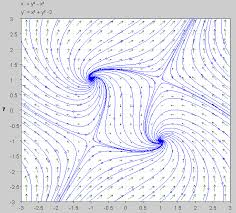
\includegraphics[scale=0.4]{vectorField.jpg}
\end{center}

% Draw pretty picture of vector field

The reason why this is true is fairly clever. Since $x + v(x) \in \mathbf{D}^n$, $v$ cannot grow too fast at the boundary, and so we may watch $v$ evolve for a small amount of time. Since no point is fixed, this tears a hole in the disk. But this evolution continuously deforms the disk, and continuous maps cannot tear holes.

\begin{theorem}
    Any map $f: \mathbf{D}^n \to \mathbf{D}^n$ has a fixed point.
\end{theorem}
\begin{proof}
Define the map $F(x,y)$ of two variables on the unit disk, which projects $x$ and $y$ to the point on the boundary of the disk obtained by following the arrow between $x$ and $y$. This is well defined and continuous for $x \neq y$. Let $f$ be a continous function such that $f(x) \neq x$ in $\mathbf{D}^n$. Then, consider the map
%
\[ F(x,f(x)) \]
%
This is a retraction of $\mathbf{D}^n$ onto $S^{n-1}$, for if $x \in S^{n-1}$, then we may let $\lambda = 0$. We prove on the homework that this induces an injective homomorphism from $H(\mathbf{S}^{n-1})$ to $H(\mathbf{D}^n)$. But since $\mathbf{D}^n$ is contractible, this would imply that the homology of $\mathbf{S}^{n-1}$ is trivial, and we know this not to be true.
\end{proof}

\section{Applications to Hex}

The fixed point theorem has suprising applications in odd little corners of mathematics, such as game theory, mathematical finance, differential equations (as we have seen), matrix theory, etc. Some applications actually give us some insight back into the theorem, and we will show one here, which shows the fixed point theorem from combinatorially.

Hex is a two player game played with each player placing pieces of their color on a board of hexagonal tiles, like so
%
\begin{center}
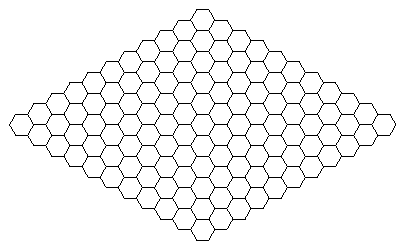
\includegraphics[scale=0.4]{hex.png}
\end{center}
%
The aim of the game is to build a path from one of your diagonal sides to your other. It's become famous among mathematicians, like the snake lemma has, because it's been in a movie. But what's a board game doing in my talk? What does the game of Hex have to do with homology theory? The trick is to take the adjacency graph on which we are {\it really} playing the game, giving us the lattice

\begin{center}
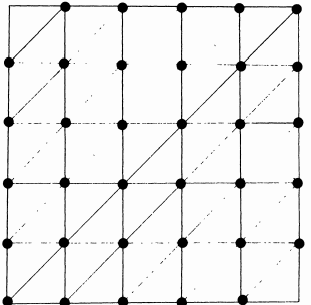
\includegraphics[scale=0.4]{lattice.png}
\end{center}

Notice that this graph gives us a {\it triangulation} of the hex board, which is homeomorphic to the unit disk. Thus facts about the combinatorial nature of the unit disk should give us insight into hex, and insight into hex might give us insight into the topology of the unit disk.

Hex was invented by John Nash when he was bored in his university dorm one night. Thus the game is also known as Nash, or John, also called that because the first few games of Hex were played on the mosaic of the dorm's bathroom floor. But John managed to turn his game into actual research, by proving the seemingly trivial theorem

\begin{theorem}
    No game of Hex can end in a draw. That is, if every tile on a hex board is filled with black or white pieces, then there is either a winning black path, or a winning left path.
\end{theorem}

If we see the game board as a river, then the only way to block a river is to build a dam between the rivers edges, so if the river does not flow through the dam, then there must be a path from one side of the river to the other. We will show that this theorem is in fact equivalent to the fixed point theorem. What's more, since this theorem will relate to the combinatorial nature of the unit disk rather than the singular nature, it will give us a constructive method to find the fixed point of the map.

\begin{theorem}
    Each map $f: I^2 \to I^2$ has a fixed point.
\end{theorem}
\begin{proof}
    The domain is compact, so it suffices to prove that for each $\varepsilon$, there is $x$ such that $\| f(x) - x \| < \varepsilon$. $f$ is also uniformly continuous, so there is $\delta$ such that if $\| x - y \| < \delta$, $\| f(x) - f(y) \|_1 < \varepsilon$. Consider the Hex board with $k^2$ tiles, where $1/k < \delta$, labelled $(1,1)$ to $(k,k)$. Let $f = (f_1, f_2)$. Place black stones on tiles $z$ where $| f_1(z/k) - z_1/k | > \varepsilon$, and white stones on tiles $z$ where $| f_2(z/k) - z_2/k | > \varepsilon$. Label the stones with positive values if $f_i(z/k) - z_i/k$ is positive, else label them with negative values. We must prove these sets are not a cover of the board. By uniform continuity, positive stones are never adjacent to negative stones of the same color. What's more, there are no positive black stones on the east side of the board, and no negative black stones on the west side of the board. If $(x_1, \dots, x_n)$ was a path of black stones from east to west, then we have argued it either has only positive stones or only negative stones. But then the path cannot meet both east and west. Similarily, there is no winning path of white stones, so Nash's theorem implies that the stones do not cover the board -- i.e. there is a point $z$ such that $\| f(z/k) - z/k \| \leq 2 \varepsilon$.
\end{proof}

This proof is easily generalize to higher dimensions by taking finer tilings. Now let us show no hex game ends in a draw.

\begin{proof}
    Consider any map $f$ from the tiles of a hex board to $\mathbf{R}^2$. Then this map extends to a continuous map on $I^2$, by taking linear combinations of the function on the simplices. In barycentric coordinates,
    %
    \[ f(\lambda_1 x_1 + \lambda_2 x_2 + \lambda_3 x_3) = \lambda_1 f(e_1) + \lambda_2 f(e_2) + \lambda_3 f(e_3) \]
    %
    Partition a hex board into two sets $H$ and $V$. Let $W$ be the all vertices connected to the west side of the board by a path in $H$, and let $W^c = H - W$. Define $S$ and $S^c$ similarily. It is clear that $W$ and $W^c$ contain no adjacent vertices, and the same is true of $S$ and $S^c$. Assume that $W$ contains no vertices on the east side of the table, and $S$ no vertices on the north side. Define
    %
    \[ f(z) = \begin{cases} z + (1,0) & z \in W \\ z - (1,0) & z \in W^c \\ z + (0,1) & z \in S \\ z - (0,1) & z \in S \end{cases} \]
    %
    and extend it to the complex on $[1,k] \times [1,k]$. On each triangle with vertices $x$, $y$, and $z$, $f$ has a fixed point in the triangle if and only if the convex hull of $f(x) - x$, $f(y) - y$, and $f(z) - z$ contains the origin, for
    %
    \[ f(\lambda_1 x + \lambda_2 y + \lambda_3 z) = \lambda_1 f(x) + \lambda_2 f(y) + \lambda_2 f(z) \]
    %
    This is a fixed point if and only if
    %
    \[ \lambda_1 (f(x) - x) + \lambda_2 (f(y) - y) + \lambda_3 (f(z) - z) = 0 \]
    %
    The fixed point theorem implies such a triangle must exist. But it is clear that such a triangle does not exist according to our mapping, for $W$ and $W^c$ are never adjacent, and the same for $S$ and $S^c$.
\end{proof}

\section{The Jordan Curve Theorem}

As with the fixed point theorem, the proof the Jordan Curve Theorem also pops out of nowhere, after a bit of fairly abstract nonsense.

\begin{theorem}
    If $X \subset S^n$ is homeomorphic to $S^k$, for $k < n$, then $\widetilde{H_{n-k-1}}(S^n - X) = \mathbf{Z}$, and is zero otherwise.
\end{theorem}
\begin{proof}
    We prove by induction on $k$. If $k = 0$, then $S^n - X$ is homeomorphic to $\mathbf{R}^n - \{ 0 \}$ homotopic to $S^{n-1}$, and $H'_{n-1}(S^{n-1}) = \mathbf{Z}$, and is zero everywhere else. Otherwise write $X = A \cup B$, where $A$ is the upper hemisphere of $S^k$, and $B$ the lower hemisphere (so $A \cap B$ is homeomorphic to $S^{k-1}$). Then $C = A \cap B$ is homeomorphic to $S^{k-1}$. We then apply Mayer Vietoris, for $M = S^n - A$, $N = S^n - B$, where
    %
    \[ M \cap N = S^n - X\ \ \ \ \ M \cup N = S^n - C \]
    %
    obtaining the long exact sequence
    %
    \[ \dots H'_i(M) \oplus H'_i(N) \to H'_i(S^n - C) \to H'_{i-1}(S^n - X) \to H_{i-1}(M) \oplus H'_{i-1}(N) \dots \]
    %
    Assuming $H'_i(M) \cong H'_i(N) \cong (0)$ for each $i$, so that
    %
    \[ H'_i(S^n - C) \cong H'_{i-1}(S^n - X) \]
    %
    So $H'_i(S^n - X) = \mathbf{Z}$ for $i+1 = n-(k-1)-1$, which occurs when $i = n-k-1$, and is zero otherwise.
\end{proof}

Thus we now need to prove

\begin{lemma}
    If $X \subset S^n$ is homeomorphic to $I^k$, then $H'_i(S^n - X) = 0$ for all $i$.
\end{lemma}
\begin{proof}
    Remark: The theorem makes intuitive sense, for if we remove a set $X$ which behaves like a point from $S^n$, then it makes sense that $S^n - X$ behaves like $\mathbf{R}^n$.

    We prove by induction. For $k = 0$, $X$ is a point, and $S^n - X$ is homeomorphic to $\mathbf{R}^n$, which contracts to a point. Otherwise, let $A \subset X$ correspond to the lower half of the $k$-cube, and $B$ the upper half. $C = A \cap B$ is then homeomorphic to $I^{k-1}$. If we let $M = S^n - A$, $N = S^n - B$, then
    %
    \[ M \cap N = S^n - X\ \ \ \ \ M \cup N = S^n - C \]
    %
    Mayer Vietoris then tells us by induction that
    %
    \[ H'_i(S^n - X) \cong H'_i(M) \oplus H'_i(N) \]
    %
    And this isomorphism is induced by the inclusions of $S^n - X$ into $M$ and $N$. Thus if $\alpha$ is an $i$ cycle in $S^n - X$ not homologous to zero, then it is not homologous to zero in $M$ or $N$. We may continue this process by splitting $M$ or $N$ into two pieces and taking isomorphisms, Showing that $\alpha$ is an $i$ cycle in sets
    %
    \[ S^n - X_1 \supset S^n - X_2 \supset S^n - X_3 \supset \dots \]
    %
    which converge to a set of the form $S^n - Y$, where $Y$ is homeomorphic to a slit $I^{k-1}$. We know that $\alpha = d \beta$ for some $\beta$ by induction. $\beta$ is a finite combination of simplices which do not come close to the slit. Since the image of the simplices does not touch $Y$, and the union of the images are compact, we see that $\beta$ is a chain in some $S^n - X_k$, contradicting that $\alpha$ is not homologous to zero.
\end{proof}

\begin{corollary}
    If $X \subset \mathbf{R}^{n+1}$ is homeomorphic to $S^n$, then it separates $n+1$ space into two components, and $X$ is the boundary of both.
\end{corollary}
\begin{proof}
    The number of components of the one point compactification of $X$ in $\mathbf{R}^{n+1}$ is equal to the number of components in the one-point compactification $S^n$, since the point at infinity has a connected neighbourhood which does not intersect $X$. Thus the number of components is the rank of $H_0'(S^{n+1} - X)$ plus one, and $H_0'(S^{n+1} - X) = \mathbf{Z}$, so there are two components in the space.

    To show that $X$ is the boundary of the two components $U$ and $V$ of $S^{n+1} - X$, pick $x \in X$, and let $W$ be an open neighbourhood of $x$. Pick a small enough closed ball $B$ in $X$ such that $B \subset W$, and let $B'$ be the closure of the other half of the sphere, also homeomorphic to a ball. Then $S^n - B'$ is path connected, as we computed the reduced homology in the last lemma, so we may pick a path $\lambda$ from a point $p \in U$ to a point $q \in V$. Necessarily, this path must cross through $X$, but then it also cross through $B$. Let $t$ be the smallest number such that $\lambda(t) \in B$. Then $t > 0$, and the path lies in $U$ for all smaller $t$, showing that there are $x \in U$ which are as closed to $B$ as could be desired, and hence there are some $x \in W$. Similarily, if we let $t$ be the largest number such that $\lambda(t) \in B$, we find points $y \in V$ that are also in $W$. Thus $x$ is in the boundary of both $U$ and $V$.
\end{proof}

In $\mathbf{R}^n$, one component of $S^n - X$ will be bounded, the other unbounded. We denote the first by the interior $\text{Int}(X)$, the second by the exterior $\text{Ext}(X)$.

\section{Invariance of Domain}

There is a certain application of the Jordan curve theorem which is very useful.

\begin{theorem}[Invariance of Domain]
    Every injective map from an open subset of $\mathbf{R}^n$ to $\mathbf{R}^n$ is open.
\end{theorem}

This reduces to

\begin{prop}
    If $f: B^n \to \mathbf{R}^n$ is continuous, then $f(B^n)$ is open.
\end{prop}
\begin{proof}
    Let $x$ be in $B^n$. Let $D$ be a closed ball around $x$. Then $\partial D \cong S^{n-1}$, and $\text{Int}(D) = D^\circ$. By compactness,
    %
    \[ f(\partial D) \cong \partial D\ \ \ \ f(D) \cong D \]
    %
    Thus $f(\partial D)$ separates $\mathbf{R}^n$ into two components. These components are
    %
    \[ \mathbf{R}^n - f(D)\ \ \ \ \ f(\text{Int}\ D) \]
    %
    the first is connected by the lemma above, the second since continuity is preserved by continuous maps. These maps are the components since they cover $\mathbf{R}^n - f(\partial D)$. But this implies
    %
    \[ f(\text{Int}\ \partial D) = \text{Int} f(\partial D) \]
    %
    hence $f$ is an open map.
\end{proof}

Now we see much more intuitively why certain $\mathbf{R}^n$ is not homeomorphic to $\mathbf{R}^m$ for $n \neq m$. If we have a homeomorphism from $\mathbf{R}^n$ to $\mathbf{R}^m$, for $n < m$. Then by embedding we would have a homeomorphism from $\mathbf{R}^m$ to a plane in $\mathbf{R}^n \times \mathbf{R}^{m-n}$. By invariance of domain, this plane would be open, but we know the plane to be closed, so the whole ruse of a homeomorphism is impossible.

\end{document}

Mathematically, we have
%
\[ F(x,y) = x + \lambda (y - x) \]
%
where $\lambda > 0$ is the unique number such that
%
\[ \| x + \lambda(y - x) \|^2 = 1 \]
%
To find this $\lambda$, we solve the equation
%
\[ (\| x \|^2 - 1) + 2 \lambda \langle x, y - x \rangle + \lambda^2 \| y - x \|^2 = 0 \]
%
which using the quadratic formula is
%
\[ \lambda = \frac{\sqrt{\langle x, y - x \rangle^2 + \| y - x \|^2 (1 - \| x \|^2)} - \langle x, y - x \rangle}{\| y - x \|^2} \]
%
So the naasasty formula is
%
\[ F(x,y) = x +  \frac{\sqrt{\langle x, y - x \rangle^2 + \| y - x \|^2 (1 - \| x \|^2)} - \langle x, y - x \rangle}{\| y - x \|^2} (y - x) \]
%
defined and continuous where $y \neq x$.